
% Acá entra el ej de RLS
		
	
	En la Figura \ref{fig:ejRLS} se muestra la convergencia de los coeficientes utilizando el algoritmo NLMS, alcanzandose finalmente los valores correctos.
	\begin{figure}[h!]
		\centering
		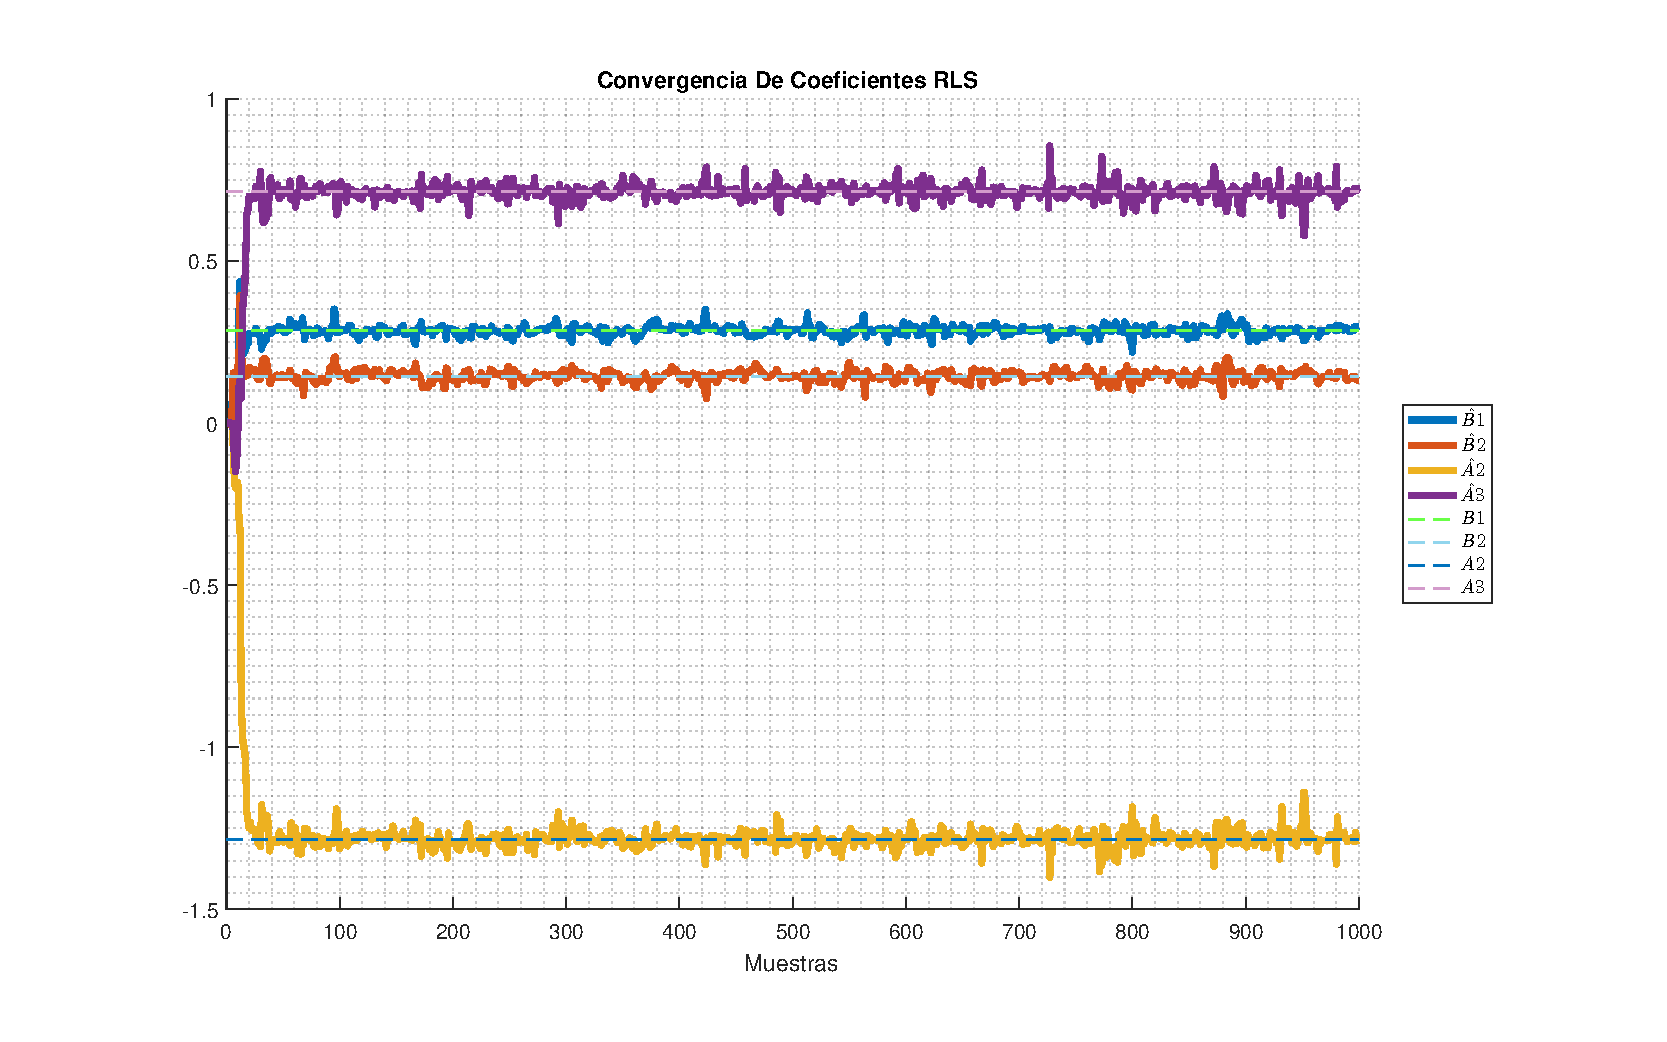
\includegraphics[width=1.0\textwidth]{graf_ejRLS.pdf}
		\caption{Convergencia de los coeficientes a partir de la estimación RLS.}
		\label{fig:ejRLS}
	\end{figure}

	\pagebreak

	\begin{figure}[h!]
		\centering
		\includegraphics[width=1.0\textwidth]{graf_LMS_vs_NLMS_vs_RLS.pdf}
		\caption{Comparación de las convergencias con LMS, NLMS y RLS.}
		\label{fig:ejRLS_comp}
	\end{figure}

	Para comparar los filtros LMS y NLMS y RLS se genera la Figura \ref{fig:ejRLS_comp} que superpone los resultados de todas las estimaciones. En ella se evidencia claramente que converge más rápido, especialmente en los coeficientes \emph{A2} y \emph{A3}.

	\begin{figure}[h!]
		\centering
		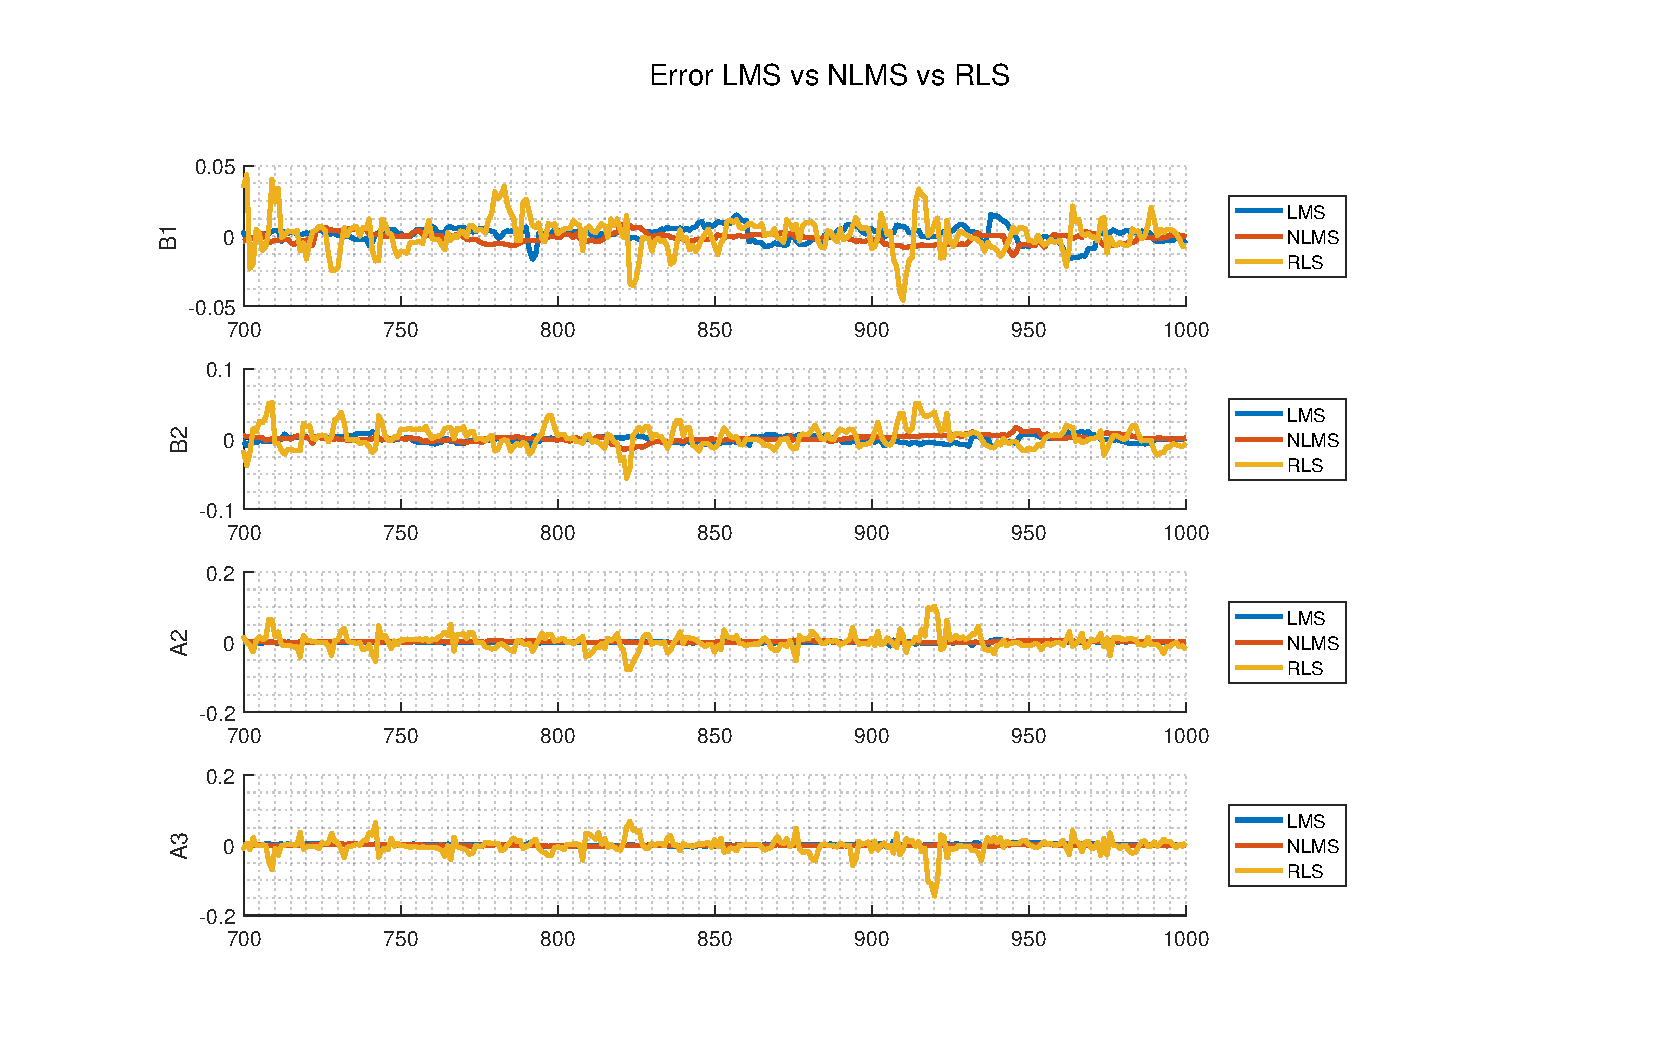
\includegraphics[width=1.0\textwidth]{graf_err_LMS_vs_NLMS_vs_RLS.pdf}
		\caption{Comparación de los valores finales de convergencia.}
		\label{fig:ejRLS_err}
	\end{figure}
	
	En la siguiente tabla, se observa la varianza de los errores de la Figura \ref{fig:ejRLS_err}. Esta vez resulta notorio que, a pesar de que RLS presenta una convergencia más rápida, la misma es más sensible al ruido.

	\begin{table}[h!]
		\centering
		\begin{tabular}{cccc}
			\toprule
			$\sigma^2$ & LMS & NLMS & RLS\\
			\midrule
			B1 & \num{2.8511e-5} & \num{1.2448e-5}  &\num{1.3543e-4}\\
			B2 & \num{2.1332e-5} & \num{1.8342e-5}  &\num{1.7859e-4}\\
			A2 & \num{4.3231e-6} & \num{2.6510e-6}  &\num{5.6104e-4}\\
			A3 & \num{7.5273e-6} & \num{2.7399e-6}  &\num{4.1981e-4}\\
			\bottomrule
		\end{tabular}
	\end{table}

	En cuanto a los resultados de la estimación de los parámetros se obtienen los siguientes resultados para el algoritmo RLS:
		\begin{table}[h!]
			\centering
			\begin{tabular}{ccc}
				\toprule
				$m$ (fija)	& $k$	& $b$\\
				\midrule
				5&\num{3.0029}&\num{1.9913}\\
				\bottomrule
			\end{tabular}
	%		\caption{Resultados de la estimación de los parámetros.}
	%		\label{tab:res_ejRLS}
		\end{table}

